\documentclass[a4paper,11pt]{article}
%%%%%%%%%%%%%%%%%%%%%%%%%%%%%%%%%%%%%%%%%%%%%%%%%%%%%%%%%%%%%%%%%%%%%%%%%%%%%%%%%%%%%%%%%%%%%%%%%%%%%%%%%%%%%%%%%%%%%%%%%%%%
\usepackage[T1]{fontenc}
\usepackage[utf8]{inputenc}
\usepackage{graphicx}
\usepackage{pdfpages} 
\usepackage{amsmath}
\usepackage{amssymb}
\usepackage{natbib}
\usepackage[dvips]{color}
\usepackage{subfigure}
\usepackage{verbatim}
\usepackage{hyperref}
\usepackage{dsfont}

\bibpunct{(}{)}{;}{a}{,}{,}

\textheight 24cm \textwidth 17cm \topmargin-2cm
%% \evensidemargin   -0.25cm
\oddsidemargin-0.2cm
%\pagestyle{empty}
\renewcommand{\baselinestretch}{1}

\begin{document}



\title{{\huge D4D Challenge} \\ \text{Commuting Dynamics 4 Change} \\ }

\author{{
				R. Lario  \footnote{rlario@paradigmatecnologico.com} 
				M. Muñoz  \footnote{mmunoz@paradigmatecnologico.com} 
				R. Abad  \footnote{rabad@paradigmatecnologico.com} 
				J. Gonzalez  \footnote{jgonzalez@paradigmatecnologico.com} 
				A. Martín  \footnote{amartin@paradigmatecnologico.com} 
				R. Maestre  \footnote{rmaestre@paradigmatecnologico.com} 
				\\\small Paradigma Labs Research Group \\\small Paradigma Tecnológico\\ \\
				E. Perez  \footnote{eperez@cchs.csic.es} 
				I. del Bosque  \footnote{idelbosque@cchs.csic.es} 
				\\\small Geographic Information Systems Unit \\\small Spanish National Research Council
				}}

\date{4-Jan-2013}
\maketitle

\begin{abstract} 
Our idea is to use the geolocation data from the antennas processing the mobile phones calls in order to know which sub-prefectures the customers have been getting around. The main goal of our project is developing spatio-temporal models to detect commuting patterns for the different sub-prefectures, including some other factors related to the region and/or time: wealth, development, infrastructure, investment, grants…

By means of GIS technology, we will be able to apply our generated models to the gathered data and to analyze their correlations over the Côte d’Ivoire surface, working with geographical layers: landcover, roads map, railways lines, water sources… Consequently, the reached conclusions from our study will be properly visualized, allowing a better explanation of the findings. With a bigger amount of data gathered for a longer period, more interesting and accurate trends could be discovered, allowing us to calculate associated coefficients.

Our analysis models will provide coherent data to support a correct urban design and will mean a monitoring tool for development, specially related to population dynamics.
In the near future, some other measures could be included. For instance, hospitals and police stations locations, their calls rate… Thus, we could know its real use, being able to improve their service to the citizens: dangerous areas, crowded hospitals…
\end{abstract}



%: ----------------------- list of figures/tables ------------------------
\newpage
\listoffigures	% print list of figures


\newpage
\setcounter{secnumdepth}{0}



%\newpage

\section{Problem description \& Hypothesis}
As we can see in the state-of-the-art section, we can extract knowledge from a mobile communication datasets, therefore in this paper the solution is built on the hypotesis of mobility patterns to predict common and well-know, geographical and time based patterns to manage roads and infrastructures in a correlated way with the results figured out.
\\
\\
The figure below shows a theoretical commuting model proposed like a main pattern. 
\\
Two peaks are modeled, $p_1$ in the range $[7, 8]$ and $p_2$ in $[17, 18]$. This first approach to modelize this dynamic set up the two peaks $p_1, p_2$ with the same weight, however, numerical results will show that the weight of each peak depends of the day of the week. A central valley is defined between $[9, 16]$, with a uniform displacement distribution.
\\
An ad-hoc mathematical model is defined in the next section in order to confirm this hypothesis; focusing, filtering and processing the main data to contrast the hypothesis.
\\
\\
The main idea behind the two main peaks in the model, $p_1, p_2$ and the central valley, is that people perform great displacement distances early in the morning i.e.: $p_1$ related with the common business activity. After the first peak $p_1$, people resides in this target destinations, working, eating, etc ..., but in a more static point of view and always performing displacements. The last point in the hypothesis approach showed by Figure~\ref{fig:commuting} is in the second peak $p_2$, when people return to his destination or the last business activites are realized.
\\
\\
The geographical behaviur of the dynamic, always mixed with the temporal component, will by contrasted by means of GIS tools in order to visualize the expansion and contraction in the main points that hypothesys shows: $p_1, p_2$ and the central valley. Exapansion when maximum displacement is reached on the first peak $p_1$ and contraction, but not quite,  when the central valley is reached. Another displacement expansion when peak $p_2$ is reached and its corresponding contraction when among $p_2$ is declining.


 
 \begin{figure}[h]
\begin{center}
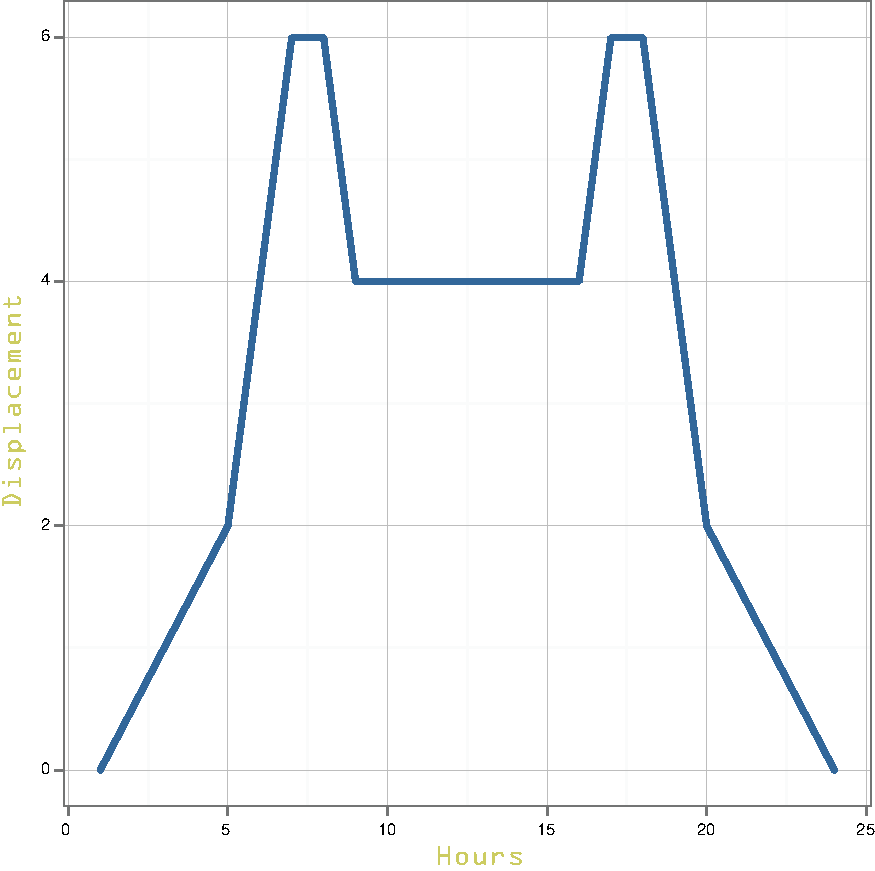
\includegraphics[scale =0.6] {results/images/common_commuting_model.pdf}
\caption{Theoretical Commuting Model}
\label{fig:commuting}
\end{center}
\end{figure} %desaparece
%\newpage

\section{Problem description \& Hypothesis}
As we can see in the state-of-the-art section, we can extract knowledge from a mobile communication datasets, therefore in this paper the solution is built on the hypotesis of mobility patterns to predict common and well-know, geographical and time based patterns to manage roads and infrastructures in a correlated way with the results figured out.
\\
\\
The figure below shows a theoretical commuting model proposed like a main pattern. 
\\
Two peaks are modeled, $p_1$ in the range $[7, 8]$ and $p_2$ in $[17, 18]$. This first approach to modelize this dynamic set up the two peaks $p_1, p_2$ with the same weight, however, numerical results will show that the weight of each peak depends of the day of the week. A central valley is defined between $[9, 16]$, with a uniform displacement distribution.
\\
An ad-hoc mathematical model is defined in the next section in order to confirm this hypothesis; focusing, filtering and processing the main data to contrast the hypothesis.
\\
\\
The main idea behind the two main peaks in the model, $p_1, p_2$ and the central valley, is that people perform great displacement distances early in the morning i.e.: $p_1$ related with the common business activity. After the first peak $p_1$, people resides in this target destinations, working, eating, etc ..., but in a more static point of view and always performing displacements. The last point in the hypothesis approach showed by Figure~\ref{fig:commuting} is in the second peak $p_2$, when people return to his destination or the last business activites are realized.
\\
\\
The geographical behaviur of the dynamic, always mixed with the temporal component, will by contrasted by means of GIS tools in order to visualize the expansion and contraction in the main points that hypothesys shows: $p_1, p_2$ and the central valley. Exapansion when maximum displacement is reached on the first peak $p_1$ and contraction, but not quite,  when the central valley is reached. Another displacement expansion when peak $p_2$ is reached and its corresponding contraction when among $p_2$ is declining.


 
 \begin{figure}[h]
\begin{center}
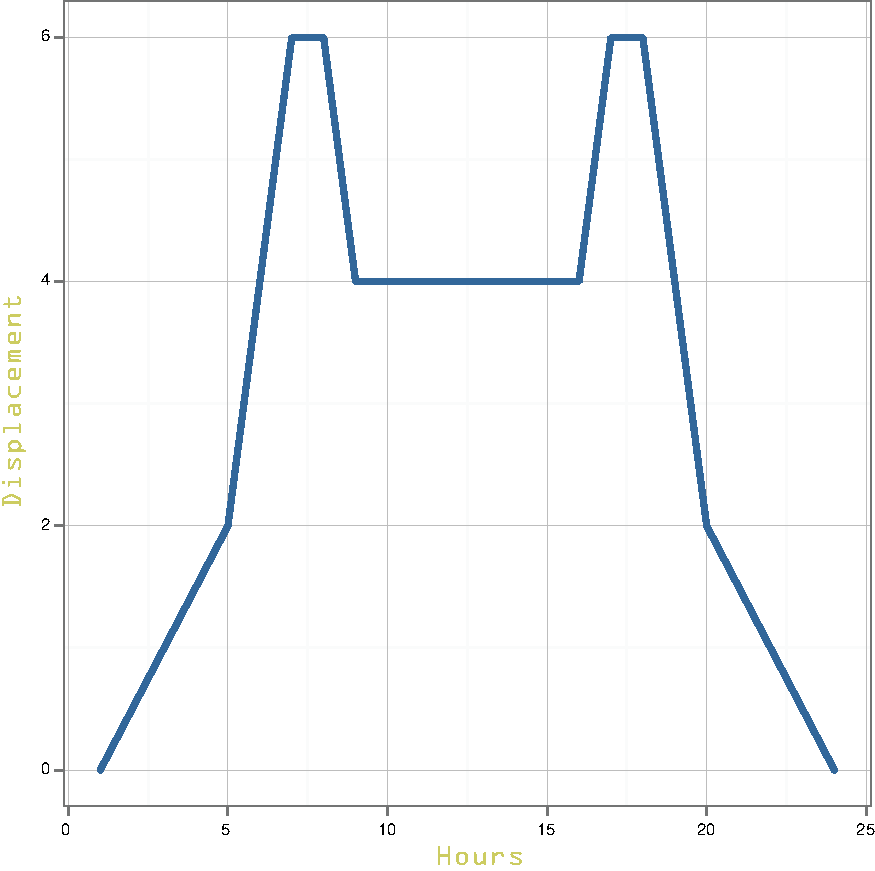
\includegraphics[scale =0.6] {results/images/common_commuting_model.pdf}
\caption{Theoretical Commuting Model}
\label{fig:commuting}
\end{center}
\end{figure} %desaparece
\newpage

\section{Problem description \& Hypothesis}
As we can see in the state-of-the-art section, we can extract knowledge from a mobile communication datasets, therefore in this paper the solution is built on the hypotesis of mobility patterns to predict common and well-know, geographical and time based patterns to manage roads and infrastructures in a correlated way with the results figured out.
\\
\\
The figure below shows a theoretical commuting model proposed like a main pattern. 
\\
Two peaks are modeled, $p_1$ in the range $[7, 8]$ and $p_2$ in $[17, 18]$. This first approach to modelize this dynamic set up the two peaks $p_1, p_2$ with the same weight, however, numerical results will show that the weight of each peak depends of the day of the week. A central valley is defined between $[9, 16]$, with a uniform displacement distribution.
\\
An ad-hoc mathematical model is defined in the next section in order to confirm this hypothesis; focusing, filtering and processing the main data to contrast the hypothesis.
\\
\\
The main idea behind the two main peaks in the model, $p_1, p_2$ and the central valley, is that people perform great displacement distances early in the morning i.e.: $p_1$ related with the common business activity. After the first peak $p_1$, people resides in this target destinations, working, eating, etc ..., but in a more static point of view and always performing displacements. The last point in the hypothesis approach showed by Figure~\ref{fig:commuting} is in the second peak $p_2$, when people return to his destination or the last business activites are realized.
\\
\\
The geographical behaviur of the dynamic, always mixed with the temporal component, will by contrasted by means of GIS tools in order to visualize the expansion and contraction in the main points that hypothesys shows: $p_1, p_2$ and the central valley. Exapansion when maximum displacement is reached on the first peak $p_1$ and contraction, but not quite,  when the central valley is reached. Another displacement expansion when peak $p_2$ is reached and its corresponding contraction when among $p_2$ is declining.


 
 \begin{figure}[h]
\begin{center}
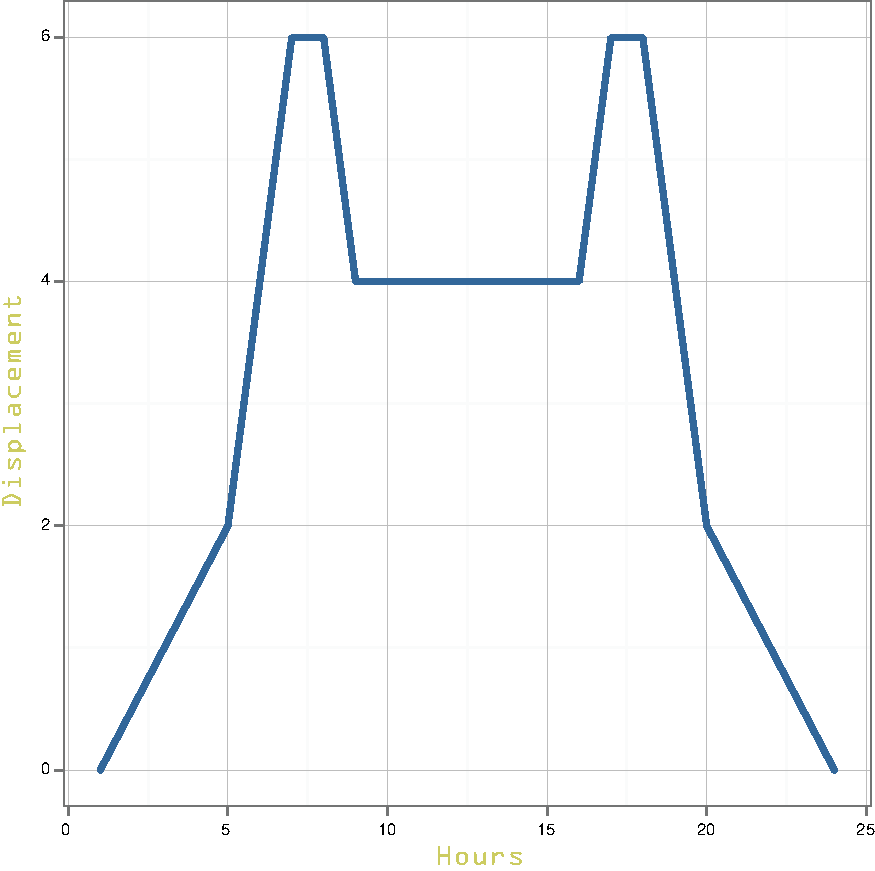
\includegraphics[scale =0.6] {results/images/common_commuting_model.pdf}
\caption{Theoretical Commuting Model}
\label{fig:commuting}
\end{center}
\end{figure} %nueva
\newpage

\section{Problem description \& Hypothesis}
As we can see in the state-of-the-art section, we can extract knowledge from a mobile communication datasets, therefore in this paper the solution is built on the hypotesis of mobility patterns to predict common and well-know, geographical and time based patterns to manage roads and infrastructures in a correlated way with the results figured out.
\\
\\
The figure below shows a theoretical commuting model proposed like a main pattern. 
\\
Two peaks are modeled, $p_1$ in the range $[7, 8]$ and $p_2$ in $[17, 18]$. This first approach to modelize this dynamic set up the two peaks $p_1, p_2$ with the same weight, however, numerical results will show that the weight of each peak depends of the day of the week. A central valley is defined between $[9, 16]$, with a uniform displacement distribution.
\\
An ad-hoc mathematical model is defined in the next section in order to confirm this hypothesis; focusing, filtering and processing the main data to contrast the hypothesis.
\\
\\
The main idea behind the two main peaks in the model, $p_1, p_2$ and the central valley, is that people perform great displacement distances early in the morning i.e.: $p_1$ related with the common business activity. After the first peak $p_1$, people resides in this target destinations, working, eating, etc ..., but in a more static point of view and always performing displacements. The last point in the hypothesis approach showed by Figure~\ref{fig:commuting} is in the second peak $p_2$, when people return to his destination or the last business activites are realized.
\\
\\
The geographical behaviur of the dynamic, always mixed with the temporal component, will by contrasted by means of GIS tools in order to visualize the expansion and contraction in the main points that hypothesys shows: $p_1, p_2$ and the central valley. Exapansion when maximum displacement is reached on the first peak $p_1$ and contraction, but not quite,  when the central valley is reached. Another displacement expansion when peak $p_2$ is reached and its corresponding contraction when among $p_2$ is declining.


 
 \begin{figure}[h]
\begin{center}
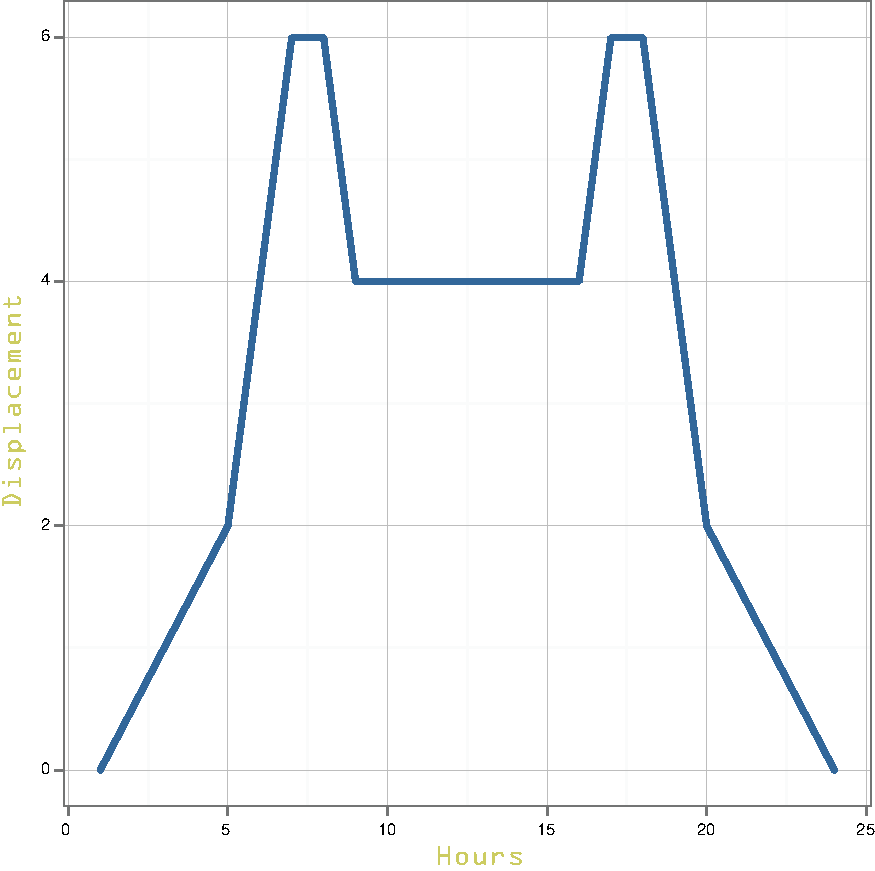
\includegraphics[scale =0.6] {results/images/common_commuting_model.pdf}
\caption{Theoretical Commuting Model}
\label{fig:commuting}
\end{center}
\end{figure} %nueva
\newpage

\section{Problem description \& Hypothesis}
As we can see in the state-of-the-art section, we can extract knowledge from a mobile communication datasets, therefore in this paper the solution is built on the hypotesis of mobility patterns to predict common and well-know, geographical and time based patterns to manage roads and infrastructures in a correlated way with the results figured out.
\\
\\
The figure below shows a theoretical commuting model proposed like a main pattern. 
\\
Two peaks are modeled, $p_1$ in the range $[7, 8]$ and $p_2$ in $[17, 18]$. This first approach to modelize this dynamic set up the two peaks $p_1, p_2$ with the same weight, however, numerical results will show that the weight of each peak depends of the day of the week. A central valley is defined between $[9, 16]$, with a uniform displacement distribution.
\\
An ad-hoc mathematical model is defined in the next section in order to confirm this hypothesis; focusing, filtering and processing the main data to contrast the hypothesis.
\\
\\
The main idea behind the two main peaks in the model, $p_1, p_2$ and the central valley, is that people perform great displacement distances early in the morning i.e.: $p_1$ related with the common business activity. After the first peak $p_1$, people resides in this target destinations, working, eating, etc ..., but in a more static point of view and always performing displacements. The last point in the hypothesis approach showed by Figure~\ref{fig:commuting} is in the second peak $p_2$, when people return to his destination or the last business activites are realized.
\\
\\
The geographical behaviur of the dynamic, always mixed with the temporal component, will by contrasted by means of GIS tools in order to visualize the expansion and contraction in the main points that hypothesys shows: $p_1, p_2$ and the central valley. Exapansion when maximum displacement is reached on the first peak $p_1$ and contraction, but not quite,  when the central valley is reached. Another displacement expansion when peak $p_2$ is reached and its corresponding contraction when among $p_2$ is declining.


 
 \begin{figure}[h]
\begin{center}
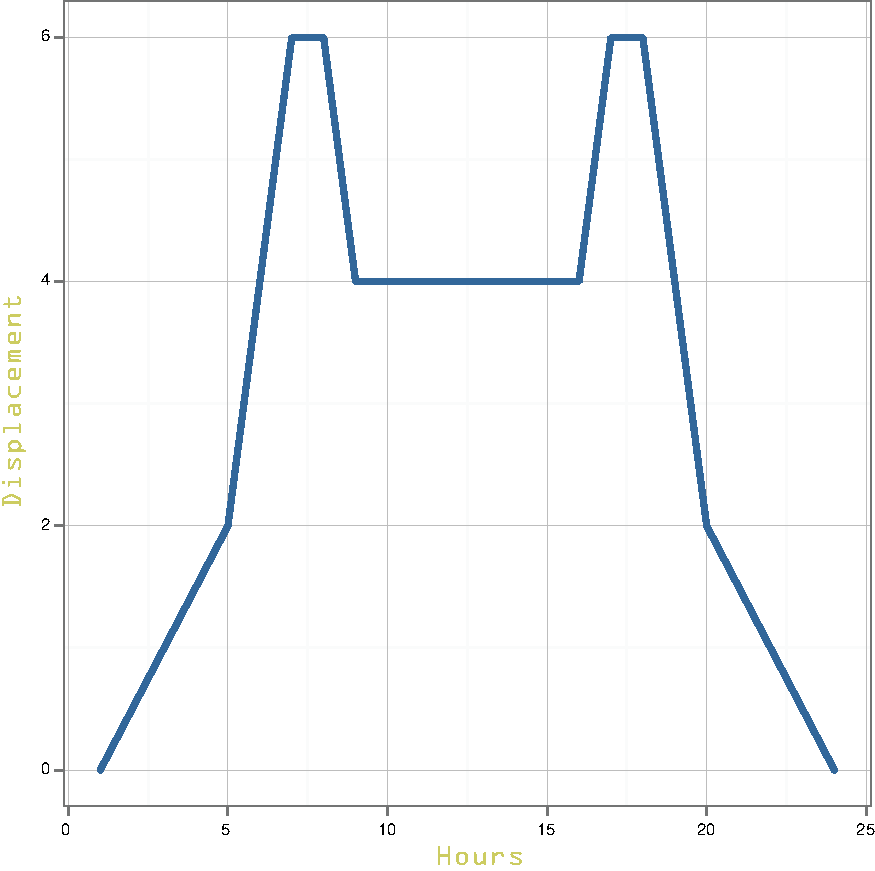
\includegraphics[scale =0.6] {results/images/common_commuting_model.pdf}
\caption{Theoretical Commuting Model}
\label{fig:commuting}
\end{center}
\end{figure} %nueva
\newpage

\section{Problem description \& Hypothesis}
As we can see in the state-of-the-art section, we can extract knowledge from a mobile communication datasets, therefore in this paper the solution is built on the hypotesis of mobility patterns to predict common and well-know, geographical and time based patterns to manage roads and infrastructures in a correlated way with the results figured out.
\\
\\
The figure below shows a theoretical commuting model proposed like a main pattern. 
\\
Two peaks are modeled, $p_1$ in the range $[7, 8]$ and $p_2$ in $[17, 18]$. This first approach to modelize this dynamic set up the two peaks $p_1, p_2$ with the same weight, however, numerical results will show that the weight of each peak depends of the day of the week. A central valley is defined between $[9, 16]$, with a uniform displacement distribution.
\\
An ad-hoc mathematical model is defined in the next section in order to confirm this hypothesis; focusing, filtering and processing the main data to contrast the hypothesis.
\\
\\
The main idea behind the two main peaks in the model, $p_1, p_2$ and the central valley, is that people perform great displacement distances early in the morning i.e.: $p_1$ related with the common business activity. After the first peak $p_1$, people resides in this target destinations, working, eating, etc ..., but in a more static point of view and always performing displacements. The last point in the hypothesis approach showed by Figure~\ref{fig:commuting} is in the second peak $p_2$, when people return to his destination or the last business activites are realized.
\\
\\
The geographical behaviur of the dynamic, always mixed with the temporal component, will by contrasted by means of GIS tools in order to visualize the expansion and contraction in the main points that hypothesys shows: $p_1, p_2$ and the central valley. Exapansion when maximum displacement is reached on the first peak $p_1$ and contraction, but not quite,  when the central valley is reached. Another displacement expansion when peak $p_2$ is reached and its corresponding contraction when among $p_2$ is declining.


 
 \begin{figure}[h]
\begin{center}
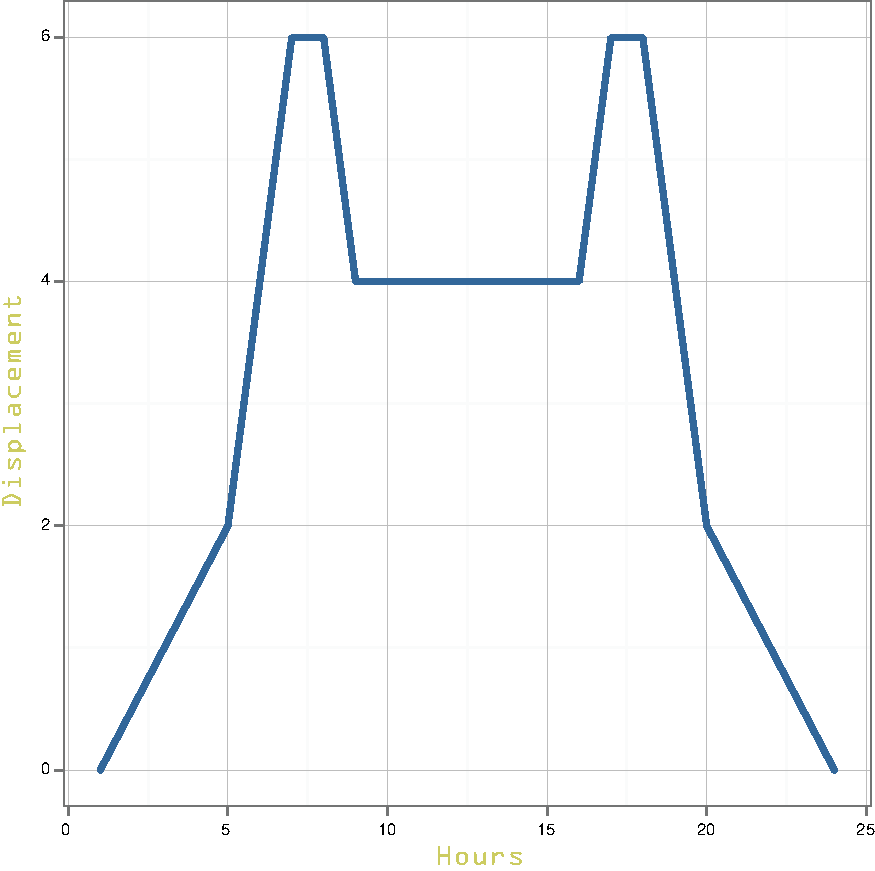
\includegraphics[scale =0.6] {results/images/common_commuting_model.pdf}
\caption{Theoretical Commuting Model}
\label{fig:commuting}
\end{center}
\end{figure}
\newpage

\section{Problem description \& Hypothesis}
As we can see in the state-of-the-art section, we can extract knowledge from a mobile communication datasets, therefore in this paper the solution is built on the hypotesis of mobility patterns to predict common and well-know, geographical and time based patterns to manage roads and infrastructures in a correlated way with the results figured out.
\\
\\
The figure below shows a theoretical commuting model proposed like a main pattern. 
\\
Two peaks are modeled, $p_1$ in the range $[7, 8]$ and $p_2$ in $[17, 18]$. This first approach to modelize this dynamic set up the two peaks $p_1, p_2$ with the same weight, however, numerical results will show that the weight of each peak depends of the day of the week. A central valley is defined between $[9, 16]$, with a uniform displacement distribution.
\\
An ad-hoc mathematical model is defined in the next section in order to confirm this hypothesis; focusing, filtering and processing the main data to contrast the hypothesis.
\\
\\
The main idea behind the two main peaks in the model, $p_1, p_2$ and the central valley, is that people perform great displacement distances early in the morning i.e.: $p_1$ related with the common business activity. After the first peak $p_1$, people resides in this target destinations, working, eating, etc ..., but in a more static point of view and always performing displacements. The last point in the hypothesis approach showed by Figure~\ref{fig:commuting} is in the second peak $p_2$, when people return to his destination or the last business activites are realized.
\\
\\
The geographical behaviur of the dynamic, always mixed with the temporal component, will by contrasted by means of GIS tools in order to visualize the expansion and contraction in the main points that hypothesys shows: $p_1, p_2$ and the central valley. Exapansion when maximum displacement is reached on the first peak $p_1$ and contraction, but not quite,  when the central valley is reached. Another displacement expansion when peak $p_2$ is reached and its corresponding contraction when among $p_2$ is declining.


 
 \begin{figure}[h]
\begin{center}
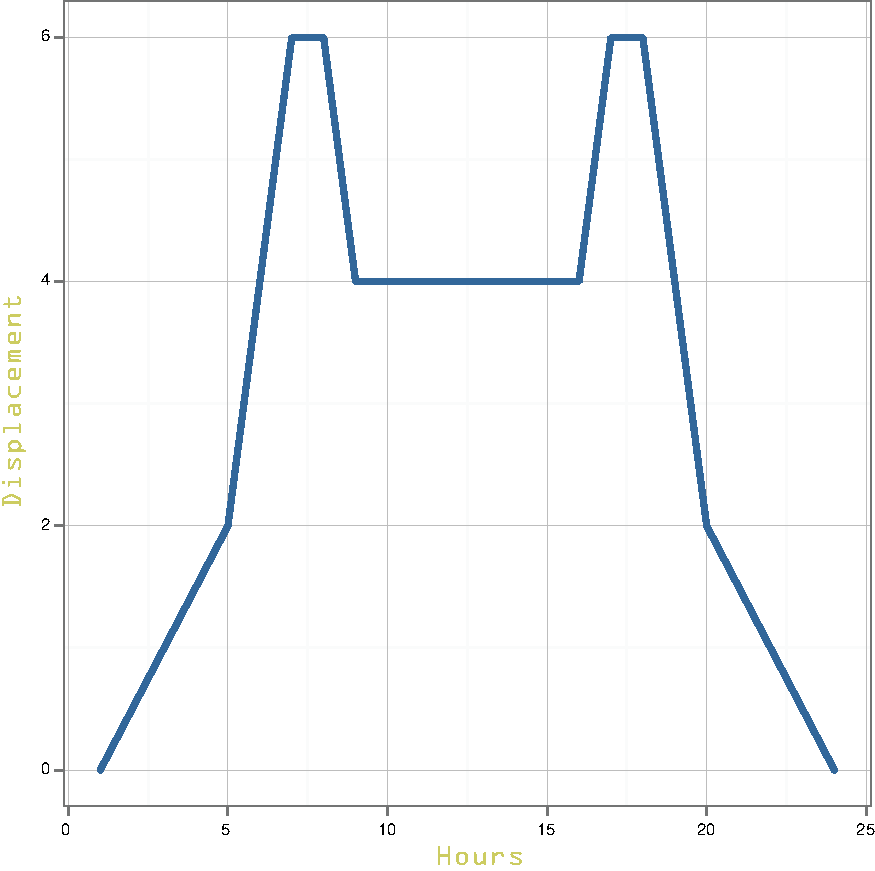
\includegraphics[scale =0.6] {results/images/common_commuting_model.pdf}
\caption{Theoretical Commuting Model}
\label{fig:commuting}
\end{center}
\end{figure} %nueva
\newpage

\section{Problem description \& Hypothesis}
As we can see in the state-of-the-art section, we can extract knowledge from a mobile communication datasets, therefore in this paper the solution is built on the hypotesis of mobility patterns to predict common and well-know, geographical and time based patterns to manage roads and infrastructures in a correlated way with the results figured out.
\\
\\
The figure below shows a theoretical commuting model proposed like a main pattern. 
\\
Two peaks are modeled, $p_1$ in the range $[7, 8]$ and $p_2$ in $[17, 18]$. This first approach to modelize this dynamic set up the two peaks $p_1, p_2$ with the same weight, however, numerical results will show that the weight of each peak depends of the day of the week. A central valley is defined between $[9, 16]$, with a uniform displacement distribution.
\\
An ad-hoc mathematical model is defined in the next section in order to confirm this hypothesis; focusing, filtering and processing the main data to contrast the hypothesis.
\\
\\
The main idea behind the two main peaks in the model, $p_1, p_2$ and the central valley, is that people perform great displacement distances early in the morning i.e.: $p_1$ related with the common business activity. After the first peak $p_1$, people resides in this target destinations, working, eating, etc ..., but in a more static point of view and always performing displacements. The last point in the hypothesis approach showed by Figure~\ref{fig:commuting} is in the second peak $p_2$, when people return to his destination or the last business activites are realized.
\\
\\
The geographical behaviur of the dynamic, always mixed with the temporal component, will by contrasted by means of GIS tools in order to visualize the expansion and contraction in the main points that hypothesys shows: $p_1, p_2$ and the central valley. Exapansion when maximum displacement is reached on the first peak $p_1$ and contraction, but not quite,  when the central valley is reached. Another displacement expansion when peak $p_2$ is reached and its corresponding contraction when among $p_2$ is declining.


 
 \begin{figure}[h]
\begin{center}
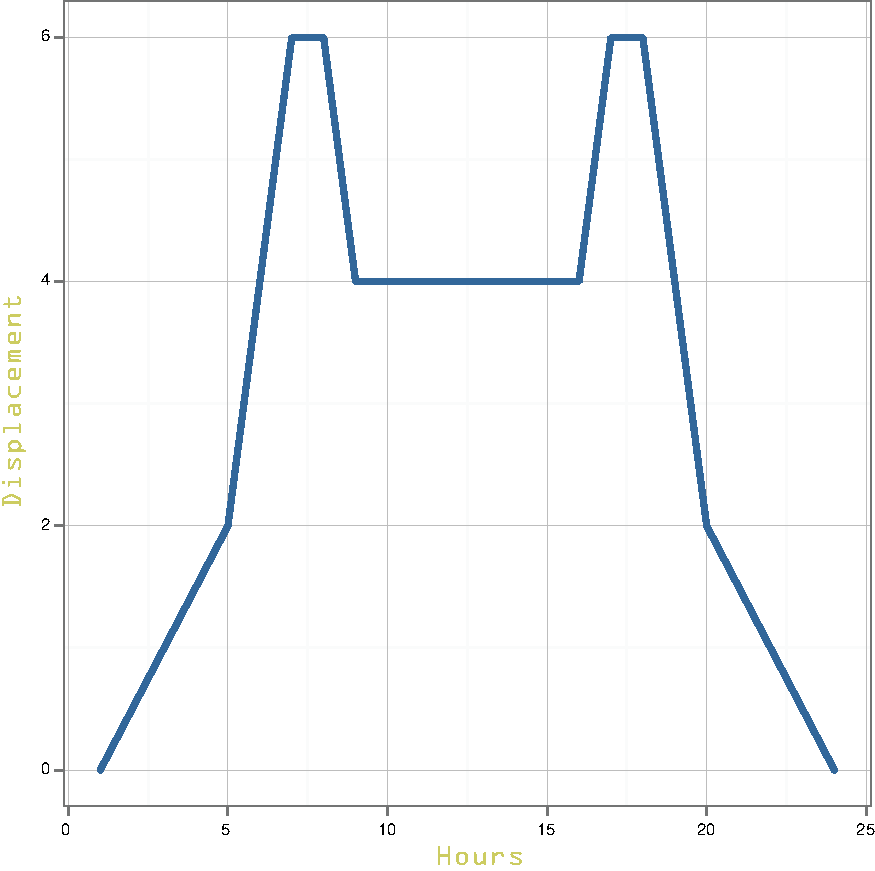
\includegraphics[scale =0.6] {results/images/common_commuting_model.pdf}
\caption{Theoretical Commuting Model}
\label{fig:commuting}
\end{center}
\end{figure}
%\newpage

\section{Problem description \& Hypothesis}
As we can see in the state-of-the-art section, we can extract knowledge from a mobile communication datasets, therefore in this paper the solution is built on the hypotesis of mobility patterns to predict common and well-know, geographical and time based patterns to manage roads and infrastructures in a correlated way with the results figured out.
\\
\\
The figure below shows a theoretical commuting model proposed like a main pattern. 
\\
Two peaks are modeled, $p_1$ in the range $[7, 8]$ and $p_2$ in $[17, 18]$. This first approach to modelize this dynamic set up the two peaks $p_1, p_2$ with the same weight, however, numerical results will show that the weight of each peak depends of the day of the week. A central valley is defined between $[9, 16]$, with a uniform displacement distribution.
\\
An ad-hoc mathematical model is defined in the next section in order to confirm this hypothesis; focusing, filtering and processing the main data to contrast the hypothesis.
\\
\\
The main idea behind the two main peaks in the model, $p_1, p_2$ and the central valley, is that people perform great displacement distances early in the morning i.e.: $p_1$ related with the common business activity. After the first peak $p_1$, people resides in this target destinations, working, eating, etc ..., but in a more static point of view and always performing displacements. The last point in the hypothesis approach showed by Figure~\ref{fig:commuting} is in the second peak $p_2$, when people return to his destination or the last business activites are realized.
\\
\\
The geographical behaviur of the dynamic, always mixed with the temporal component, will by contrasted by means of GIS tools in order to visualize the expansion and contraction in the main points that hypothesys shows: $p_1, p_2$ and the central valley. Exapansion when maximum displacement is reached on the first peak $p_1$ and contraction, but not quite,  when the central valley is reached. Another displacement expansion when peak $p_2$ is reached and its corresponding contraction when among $p_2$ is declining.


 
 \begin{figure}[h]
\begin{center}
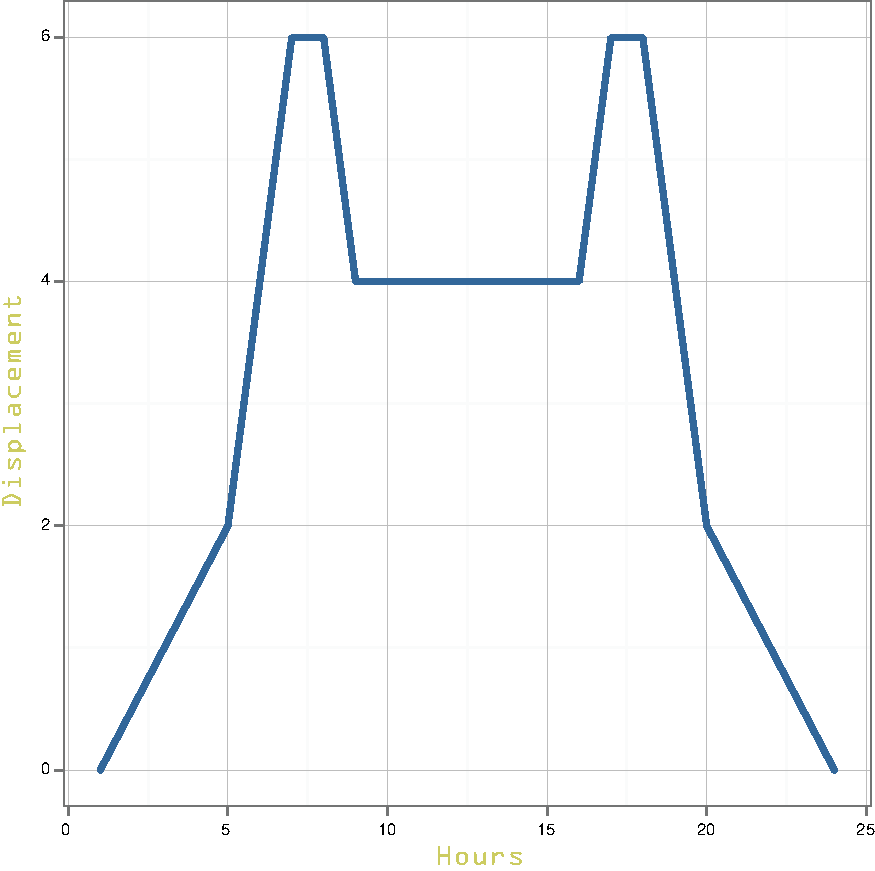
\includegraphics[scale =0.6] {results/images/common_commuting_model.pdf}
\caption{Theoretical Commuting Model}
\label{fig:commuting}
\end{center}
\end{figure} %desaparece
\newpage

\section{Problem description \& Hypothesis}
As we can see in the state-of-the-art section, we can extract knowledge from a mobile communication datasets, therefore in this paper the solution is built on the hypotesis of mobility patterns to predict common and well-know, geographical and time based patterns to manage roads and infrastructures in a correlated way with the results figured out.
\\
\\
The figure below shows a theoretical commuting model proposed like a main pattern. 
\\
Two peaks are modeled, $p_1$ in the range $[7, 8]$ and $p_2$ in $[17, 18]$. This first approach to modelize this dynamic set up the two peaks $p_1, p_2$ with the same weight, however, numerical results will show that the weight of each peak depends of the day of the week. A central valley is defined between $[9, 16]$, with a uniform displacement distribution.
\\
An ad-hoc mathematical model is defined in the next section in order to confirm this hypothesis; focusing, filtering and processing the main data to contrast the hypothesis.
\\
\\
The main idea behind the two main peaks in the model, $p_1, p_2$ and the central valley, is that people perform great displacement distances early in the morning i.e.: $p_1$ related with the common business activity. After the first peak $p_1$, people resides in this target destinations, working, eating, etc ..., but in a more static point of view and always performing displacements. The last point in the hypothesis approach showed by Figure~\ref{fig:commuting} is in the second peak $p_2$, when people return to his destination or the last business activites are realized.
\\
\\
The geographical behaviur of the dynamic, always mixed with the temporal component, will by contrasted by means of GIS tools in order to visualize the expansion and contraction in the main points that hypothesys shows: $p_1, p_2$ and the central valley. Exapansion when maximum displacement is reached on the first peak $p_1$ and contraction, but not quite,  when the central valley is reached. Another displacement expansion when peak $p_2$ is reached and its corresponding contraction when among $p_2$ is declining.


 
 \begin{figure}[h]
\begin{center}
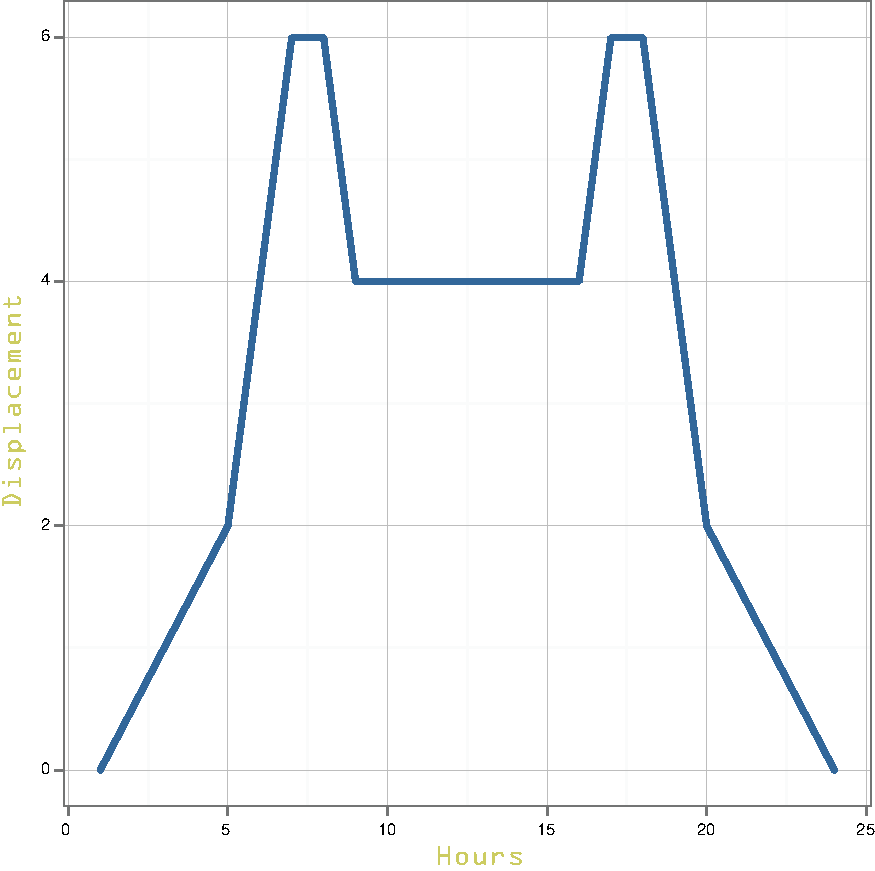
\includegraphics[scale =0.6] {results/images/common_commuting_model.pdf}
\caption{Theoretical Commuting Model}
\label{fig:commuting}
\end{center}
\end{figure}

%ggplot(data) + geom_path( aes(x=HOURS, y=RATIO_MEDIAN_DISTANCE2DYNAMIC_USERS, colour= DYNAMIC_USERS, size=DYNAMIC_USERS), lineend = "round", linejoin = "bevel")

\newpage
\bibliographystyle{plainnat}
\bibliography{biblio}

\end{document}



